%%%%%%%%%%%%%%%%%%%%%%%%%%%%%%%%%%%%%%%%%%%%%%%%%%%%%%%%
%%
\chapter{The Recipes}
\label{ch:the_recipes}
%%
%%%%%%%%%%%%%%%%%%%%%%%%%%%%%%%%%%%%%%%%%%%%%%%%%%%%%%%%


%%%%%%%%%%%%%%%%%%%%%%%%%%%%%%%%%%%%%%%%%%%%%%%%%%%%%%%%
%%
\ifdevguide
\section{General}
\label{ch:the_recipes:gen_layout}
%%
%%%%%%%%%%%%%%%%%%%%%%%%%%%%%%%%%%%%%%%%%%%%%%%%%%%%%%%%

The recipes are designed to have a layout that minimizes repetition and looks familiar between recipes. Much of the functionality in the recipes is used in multiple recipes and thus appears in functional form as opposed to be redefined in each and every recipe.

Some of this functionality was explained in section \ref{ch:rules:drs_specific}, explicitly the following:
\begin{itemize}
	\item the logging functionality -- logging to both screen and file (Section \ref{ch:rules:drs_specific:logger}).
	\item the parameter dictionary -- specialized dictionary object to store key value pairs with a source attached to each, i.e. to keep track of where key value pairs are defined and changed (Section \ref{ch:rules:drs_specific:param_dict}).
	\item the configuration error and exception class -- a special error and exception handling class for dealing with the configuration files and parameters associated with them (Section \ref{ch:rules:drs_specific:config_error}).
\end{itemize}

\vspace{0.5cm}
\noindent In addition to these each recipe is defined with a function itself (the \progMAIN function), to enable calling of said recipe from inside other python scripts (i.e. for batch runs).

\vspace{0.5cm}
\noindent The rest of this section details the different parts of the recipes.

% -------------------------------------------------------
\subsection{The setup procedures}
\label{ch:the_recipes:gen_layout:setup}
% -------------------------------------------------------


The first functionality of any recipe \progMAIN function is to setup the recipe for running. This is done in three main steps (recipes may or may not use all three steps).

\begin{enumerate}
	\item \spirouStartup.Begin() -- Loads the initial parameters from the main configuration file.

	\item \spirouStartup.LoadArguments() -- Loads parameters from run time arguments (in default configuration or custom argument configuration, see sections \ref{ch:the_recipes:gen_layout:standard_recipes} and \ref{ch:the_recipes:gen_layout:custom_arguments})
	\begin{note}
	Required prefixes (such as `dark\_dark', `fp\_fp', `flat\_dark') can be set here to cause an exception if the filenames provided to not have one or more of these prefixes (useful in controlling which files are allowed to be used in the recipe).
	\end{note}

	\item \spirouStartup.InitialFileSetup() -- Pushes values such as `log\_opt', `fitsfilename', `arg\_night\_name' into the main constant parameter dictionary `p' and loads the calibration database, if present.
\end{enumerate}

As mentioned above there are two ways to load arguments, the `default' way or the `custom' way. These are described in sections \ref{ch:the_recipes:gen_layout:standard_recipes} and \ref{ch:the_recipes:gen_layout:custom_arguments} below.

% -------------------------------------------------------
\clearpage
\newpage
\subsubsection{Standard recipes}
\label{ch:the_recipes:gen_layout:standard_recipes}
% -------------------------------------------------------

The standard way of getting arguments from the user is as follows:

\begin{cmdbox}
RECIPE_NAME.py FOLDER FILENAME1
\end{cmdbox}

\noindent with more files defined the following way:

\begin{cmdbox}
RECIPE_NAME.py FOLDER FILENAME1 FILENAME2
\end{cmdbox}

These (using \spirouStartup.LoadArguments()) are loaded in to parameters. `FOLDER' becomes \definevariable{text:arg_night_name}{arg\_night\_name}, `FILENAME1' or `FILENAME1 FILENAME2' become a python list accessed via \definevariable{text:arg_file_names}{arg\_file\_names} with the first filename also being defined as \definevariable{text:fitsfilename}{fitsfilename}. The `RECIPE\_NAME' is loaded into \definevariable{text:log_opt}{log\_opt} for use in the log.

An example standard load up can be seen in \calDARK.

\begin{cmdbox}
(*\calDARK*).py 20170710 dark_dark02d406.fits
\end{cmdbox}

\begin{pythonbox}
    # ----------------------------------------------------------------------
    # Set up
    # ----------------------------------------------------------------------
    # get parameters from config files/run time args/load paths + calibdb
    p = spirouStartup.Begin()
    p = spirouStartup.LoadArguments(p, night_name, files)
    p = spirouStartup.InitialFileSetup(p, kind='dark', prefixes=['dark_dark'])
\end{pythonbox}
\begin{note}
Here `night\_name' and `files' come from the \progMAIN definition (i.e. if called from python as a function we must have a way to get the arguments as they will not be defined at run time). As this is for \calDARK the `kind' of file is `dark' (used in logging) and the prefixes allowed for dark files are `dark\_dark' only.
\end{note}

% -------------------------------------------------------
\subsubsection{Recipes with custom arguments}
\label{ch:the_recipes:gen_layout:custom_arguments}
% -------------------------------------------------------

For custom argument recipes the way of getting arguments from the user is as follows:

\begin{cmdbox}
RECIPE_NAME.py FOLDER ARG1 ARG2 ARG3
\end{cmdbox}

In some cases the standard arguments are not sufficient for user input (i.e. for a certain recipe we may need more than just a list of file names). In this case the function \spirouStartup.LoadArguments() is used with keyword `customargs' with a valid python dictionary of key names and their respective values. The helper function \spirouStartup.GetCustomFromRuntime() can be used to construct this dictionary accessing variables from the run time. 

\begin{minipage}{\textwidth}
An example can be seen in \calCCF.
\begin{cmdbox}
(*\calCCF*).py 20170710 fp_fp02a203_e2ds_AB.fits UrNe.mas 0 10 0.1
\end{cmdbox}
\begin{pythonbox}
    # ----------------------------------------------------------------------
    # Set up
    # ----------------------------------------------------------------------
    # get parameters from config files/run time args/load paths + calibdb
    p = spirouStartup.Begin()

    # deal with arguments being None (i.e. get from sys.argv)
    pos = [0, 1, 2, 3, 4]
    fmt = [str, str, float, float, float]
    name = ['reffile', 'ccf_mask', 'target_rv', 'ccf_width', 'ccf_step']
    lname = ['input_file', 'CCF_mask', 'RV', 'CCF_width', 'CCF_step']
    req = [True, True, True, False, False]
    call = [reffile, mask, rv, width, step]
    call_priority = [True, True, True, True, True]
    # now get custom arguments
    customargs = spirouStartup.GetCustomFromRuntime(pos, fmt, name, req, call,
                                                    call_priority, lname)
    
    # get parameters from configuration files and run time arguments
    p = spirouStartup.LoadArguments(p, night_name, customargs=customargs)
\end{pythonbox}
\begin{note}
Here \calCCF requires the custom arguments `reffile', `ccf\_mask', `target\_rv', `ccf\_width' and `ccf\_step'. These must be defined in \progMAIN and must be defined in the list `call'. 

The other parameters required by \spirouStartup.GetCustomFromRuntime() are:
\begin{itemize}
	\item `pos' -- the position expected in the run time arguments (after the folder name)
	\item `fmt' -- the format expected from an argument (i.e. string or float, or integer)
	\item `name' -- the name in the parameter dictionary for each argument
	\item `lname' -- the log name (the name the user will see in the log if there is an error)
	\item `req' -- whether the argument is required (True) or optional (False)
	\item `call' -- the name from \progMAIN
	\item `call\_priority' -- whether arguments from \progMAIN overrides values from run time (most the time this will be True for use from python functions).
\end{itemize}
\end{note}
\end{minipage}



% -------------------------------------------------------
\clearpage
\newpage
\subsection{Main recipe code}
\label{ch:the_recipes:gen_layout:main_recipe_code}
% -------------------------------------------------------

After the setup proceedure the main code is run. Most heavy lifting should be done in functions and for ease of the reader/developer the main code should be kept to one line codes calling functions from the DRS python module. Many codes are reused throughout the drs a few of them are listed below:

\begin{itemize}

	\item \spirouImage.ReadImageAndCombine -- Loads \definevariable{text:fitsfilename}{fitsfilename} image and header (and if framemath define combines with all other files in \definevariable{text:arg_file_names}{arg\_file\_names}).

	\item \spirouImage.GetSigdet -- gets the \definevariable{text:sigdet}{read noise} value from the \definevariable{text:fitsfilename}{fitsfilename} header

	\item \spirouImage.GetExpTime -- gets the \definevariable{text:exptime}{exposure time} from the \definevariable{text:fitsfilename}{fitsfilename} header

	\item \spirouImage.GetGain -- gets the \definevariable{text:gain}{gain} from the \definevariable{text:fitsfilename}{fitsfilename} header.

	\item \spirouImage.CorrectForDark -- Loads the dark from the calibration database and applies it to the `data' keyword

	\item \spirouImage.ConvertToE -- Converts image from ADU/s into e- using the \definevariable{text:exptime}{exposure time} and  the \definevariable{text:gain}{gain}

	\item \spirouImage.FlipImage -- flips the image in one or both of the dimensions (using the `flipx' and `flipy' keywords)
 
	\item \spirouImage.ResizeImage -- Resizes the image based on `xlow', `xhigh', `ylow' and `yhigh' keywords

\end{itemize}


% -------------------------------------------------------
\clearpage
\newpage
\subsection{Writing to file}
\label{ch:the_recipes:gen_layout:writing_to_file}
% -------------------------------------------------------

Files are written to disk using the \spirouImage.WriteImage() function. This requires a filename (python string), a image file (the data), and a header dictionary. Most filenames are defined in \spirouConfig.Constants (see Section \ref{ch:variables:outputvariables}). The header dictionary can be taken straight from the raw \definevariable{text:fitsfilename}{fitsfilename} header (the output of \spirouImage.ReadImageAndCombine for example), but key can be added using the following commands:

\begin{itemize}
	\item \spirouImage.CopyOriginalKeys -- copies the original keys from the \definevariable{text:fitsfilename}{fitsfilename} except those keys in \definevariable{text:forbidden_keys}{forbidden keys}.

	\item \spirouImage.AddKey -- adds a single key to the header (using the header keyword list parameters, see Section \ref{ch:output_keywords}) and a value defined by the user using the `value' keyword, if not defined the default value will be used.

	\item \spirouImage.AddKey2DList -- adds a 2D list to the header (using the header keyword list parameters, see Section \ref{ch:output_keywords})
\end{itemize}

\vspace{0.5cm}
\begin{minipage}{\textwidth}
\noindent An example is shown below
\begin{pythonbox}
# ----------------------------------------------------------------------
# Save and record of image of localization with order center and keywords
# ----------------------------------------------------------------------
# log that we are saving localization file
wmsg = 'Saving FWHM information in file: {0}'
WLOG('', p['log_opt'], wmsg.format(locofits2name))

# add keys from original header file
hdict = spirouImage.CopyOriginalKeys(hdr, cdr)

# define new keys to add
hdict = spirouImage.AddKey(hdict, p['kw_version'])
hdict = spirouImage.AddKey(hdict, p['kw_CCD_SIGDET'])
hdict = spirouImage.AddKey(hdict, p['kw_LOCO_NBO'], value=rorder_num)

# write 2D list of position fit coefficients
hdict = spirouImage.AddKey2DList(hdict, p['kw_LOCO_CTR_COEFF'],
                                 values=loc['acc'][0:rorder_num])

# add quality control
hdict = spirouImage.AddKey(hdict, p['kw_drs_QC'], value=p['QC'])

# write image and add header keys (via hdict)
spirouImage.WriteImage(locofits2, width_fits, hdict)
\end{pythonbox}
\begin{note}
Here we add the original keys not in \definevariable{text:forbidden_keys}{forbidden keys} to the header dictionary `hdict' and then add \definevariable{text:kw_version}{version}, \definevariable{text:kw_ccd_sigdet}{sigdet} and \definevariable{text:kw_loco_nbo} {the number of orders localized} as single keys, add the localization centers as a 2D list and add the flag for whether the quality control was passed.
\end{note}
\end{minipage}

% -------------------------------------------------------
\clearpage
\newpage
\subsection{Quality control}
\label{ch:the_recipes:gen_layout:gen_qc}
% -------------------------------------------------------

Quality control parameters decide whether a file is written to the calibration database. They consist of a standard python if statement where the variable `passed' must be set to False if a quality control criteria fails the processed file (i.e. this is done inside the if or an else statement). As well as this a message may be passed to the log (standard output/screen and the log file), this is done by appending to `fail\_msg' which is subsequently printed for all quality control criteria that fail the test.

\vspace{0.5cm}
\begin{minipage}{\textwidth}
\noindent An example is shown below
\begin{pythonbox}
# ----------------------------------------------------------------------
# Quality control
# ----------------------------------------------------------------------
passed, fail_msg = True, []
# check that max number of points rejected in center fit is below threshold
if np.sum(loc['max_rmpts_pos']) > p['QC_LOC_MAXLOCFIT_REMOVED_CTR']:
    fmsg = 'abnormal points rejection during ctr fit ({0} > {1})'
    fail_msg.append(fmsg.format(np.sum(loc['max_rmpts_pos']),
                                p['QC_LOC_MAXLOCFIT_REMOVED_CTR']))
    passed = False
# check that max number of points rejected in width fit is below threshold
if np.sum(loc['max_rmpts_wid']) > p['QC_LOC_MAXLOCFIT_REMOVED_WID']:
    fmsg = 'abnormal points rejection during width fit ({0} > {1})'
    fail_msg.append(fmsg.format(np.sum(loc['max_rmpts_wid']),
                                p['QC_LOC_MAXLOCFIT_REMOVED_WID']))
    passed = False
# finally log the failed messages and set QC = 1 if we pass the
# quality control QC = 0 if we fail quality control
if passed:
    WLOG('info', p['log_opt'], 'QUALITY CONTROL SUCCESSFUL - Well Done -')
    p['QC'] = 1
    p.set_source('QC', __NAME__ + '/main()')
else:
    for farg in fail_msg:
        wmsg = 'QUALITY CONTROL FAILED: {0}'
        WLOG('info', p['log_opt'], wmsg.format(farg))
    p['QC'] = 0
    p.set_source('QC', __NAME__ + '/main()')
\end{pythonbox}
\begin{note}
Here we check that the maximum number of points rejected in center fit is below a threshold and check that the maximum number of points rejected in the width fit is below a threshold if either of these fail then their `fail\_msg' is logged and printed, else a message saying `quality control successful' is displayed.
\end{note}
\end{minipage}

% -------------------------------------------------------
\clearpage
\newpage
\subsection{Writing to the calibration database}
\label{ch:the_recipes:gen_layout:writing_calibdb}
% -------------------------------------------------------

The calibration database is automatically opened at the start of the recipes (see Section \ref{ch:the_recipes:gen_layout:setup}). Two commands are used to interface with the calibration database. The first \spirouCDB.PutFile() adds the file to the calibration database folder. The second (\spirouCDB.UpdateMaster) updates the \masterCALIBDBfile with the correct key (set using the `keys' keyword, e.g. `DARK' or `LOC\_AB').


\vspace{0.5cm}
\begin{minipage}{\textwidth}
\noindent An example is shown below
\begin{pythonbox}
# ----------------------------------------------------------------------
# Update the calibration database
# ----------------------------------------------------------------------
if p['QC'] == 1:
    keydb = 'LOC_' + p['fiber']
    # copy localisation file to the calibDB folder
    spirouCDB.PutFile(p, locofits)
    # update the master calib DB file with new key
    spirouCDB.UpdateMaster(p, keydb, locofitsname, hdr)
\end{pythonbox}
\begin{note}
Here we add, for example, key `LOC\_AB' or `LOC\_C' to the calibration database. The file is first put in the \definevariable{text:drs_calib_db}{calibration database folder} and then the key, filename and date/time are added to the \masterCALIBDBfile. The date/time that is used is that of the \definevariable{text:fitsfilename}{fitsfilename}.
\end{note}
\end{minipage}

% -------------------------------------------------------
\subsection{End of code}
\label{ch:the_recipes:gen_layout:end}
% -------------------------------------------------------

After all the main section is completed, the code should end with the final log statement. This is followed by a returning of the local-scope variables (via the `locals()' command), this allows the developer to have access to the local-scope of the functions on calling the function from another python script (this is used extensively in the unit test functions). For consistency this finishing message should not change and be present at the end of each recipe, thus on seeing this message the user and developer know that the recipe is finished.

\vspace{0.5cm}
\begin{minipage}{\textwidth}
\noindent An example is shown below
\begin{pythonbox}
# ----------------------------------------------------------------------
# End Message
# ----------------------------------------------------------------------
wmsg = 'Recipe {0} has been successfully completed'
WLOG('info', p['log_opt'], wmsg.format(p['program']))

return locals()
\end{pythonbox}
\end{minipage}

\clearpage
\newpage
\fi










%%%%%%%%%%%%%%%%%%%%%%%%%%%%%%%%%%%%%%%%%%%%%%%%%%%%%%%%
%%
\section{The cal\_DARK recipe}
\label{ch:the_recipes:cal_DARK_spirou}
%%
%%%%%%%%%%%%%%%%%%%%%%%%%%%%%%%%%%%%%%%%%%%%%%%%%%%%%%%%

Dark with short exposure time (~5min, to be defined during AT-4) to check if read-out noise, dark current and hot pixel mask are consistent with the ones obtained during technical night. Quality control is done automatically by the pipeline \\


% -------------------------------------------------------
\subsection{The inputs}
% -------------------------------------------------------
The input of \calDARK is as follows:
\begin{cmdbox}
cal_DARK_spirou.py  night_repository  filenames
\end{cmdbox}
\noindent or
\begin{pythonbox}
import cal_DARK_spirou
night_reposityory = '20170710'
filenames = ['dark_dark02d406.fits']
cal_DARK_spirou.main(night_repository, filenames)
\end{pythonbox}

\noindent where `night\_repository' defines \argnightname and `filenames' define the list of files in \argfilenames. All files in filenames must be valid python strings separated by a space (command line) or in a line (python). \\

\noindent Filename prefixes allowed are:
\begin{itemize}
	\item dark\_dark
\end{itemize}

% -------------------------------------------------------
\subsection{The outputs}
% -------------------------------------------------------
The outputs of \calDARK are as follows:

\begin{itemize}
\item \definevariable{text:darkfile}{darkfile} in form:
\begin{tcustomdir}
\{\reduceddir\}\{date prefix\}\_\{file\}.fits
\end{tcustomdir}

\item \definevariable{text:darkbadpixfile}{darkbadpixfile} in form:
\begin{tcustomdir}
\{\reduceddir\}\{date prefix\}\_\{file\}\_badpixel.fits
\end{tcustomdir}
\end{itemize}

\noindent where `date prefix' is constructed from \argnightname and the file name is the first file in \argfilenames.

% -------------------------------------------------------
\subsection{Summary of procedure}
% -------------------------------------------------------
\begin{enumerate}
\item adds defined `dark\_dark' files together
\item resizes the image
\item calculates the fraction of dead pixels [full, blue part, red part]
\item calculates median dark level [full, blue part, red part]
\item calculates threshold of dark level to retain
\item removes dead pixels by setting them to 0
\item does some quality control
\item updates calibDB with key "DARK"
\end{enumerate}


% -------------------------------------------------------
\subsection{Quality Control}
% -------------------------------------------------------


There are currently three quality control checks for cal\_DARK\_spirou
\begin{itemize}
\item Unexpected median dark level if: 
\begin{thighlight}
\begin{equation}
\text{Median Flux} > \text{\definevariable{text:qc_max_darklevel}{qc\_max\_darklevel}}
\end{equation}
\end{thighlight}

\item Unexpected fraction of dead pixels if: 
\begin{thighlight}
\begin{equation}
\text{Number of dead pixels} > \text{\definevariable{text:qc_max_dead}{qc\_max\_dead}}
\end{equation}
\end{thighlight}

\item Unexpected fraction of dark pixels if:
\begin{thighlight}
\begin{equation}
\text{Number of bad dark pixels} > \text{\definevariable{text:qc_max_dark}{qc\_max\_dark}}
\end{equation}
\end{thighlight}
\end{itemize}

If none of these quality control criteria are valid then the output file is passed into the \calibdb with key `DARK' for the `darkfile' and `BADPIX' for the `darkbadpixfile'.

% -------------------------------------------------------
\newpage
\subsection{Example working run}
% -------------------------------------------------------

An example run where everything worked is below:

\begin{cmdboxprintspecial}
@g20:57:30.8 -   || ***************************************** 
20:57:30.8 -   || * SPIROU \@(#) Geneva Observatory (0.0.057) 
20:57:30.8 -   || ***************************************** 
20:57:30.8 -   ||(dir_data_raw)      DRS_DATA_RAW=/scratch/Projects/spirou_py3/data/raw 
20:57:30.8 -   ||(dir_data_reduc)    DRS_DATA_REDUC=/scratch/Projects/spirou_py3/data/reduced 
20:57:30.8 -   ||(dir_calib_db)      DRS_CALIB_DB=/scratch/Projects/spirou_py3/data/calibDB 
20:57:30.8 -   ||(dir_data_msg)      DRS_DATA_MSG=/scratch/Projects/spirou_py3/data/msg 
20:57:30.8 -   ||(print_level)       PRINT_LEVEL=all         %(error/warning/info/all) 
20:57:30.8 -   ||(log_level)         LOG_LEVEL=all         %(error/warning/info/all) 
20:57:30.8 -   ||(plot_graph)        DRS_PLOT=1            %(def/undef/trigger) 
20:57:30.8 -   ||(used_date)         DRS_USED_DATE=undefined
20:57:30.8 -   ||(working_dir)       DRS_DATA_WORKING=/scratch/Projects/spirou_py3/data/tmp/
20:57:30.8 -   ||                    DRS_INTERACTIVE is not set, running on-line mode
20:57:30.8 -   ||                    DRS_DEBUG is set, debug mode level:1
20:57:30.8 -   |ipython:2d406|Now running : ipython on file(s): dark_dark02d406.fits
20:57:30.8 -   |ipython:2d406|On directory /scratch/Projects/spirou_py3/data/raw/20170710
20:57:30.8 -   |ipython:2d406|ICDP_NAME loaded from: /scratch/Projects/spirou_py3/INTROOT/config/constants_SPIROU.py
20:57:30.8 - * |ipython:2d406|Correct type of image for dark (dark_dark)
20:57:31.0 - * |ipython:2d406|Now processing Image TYPE UNKNOWN with ipython recipe
20:57:31.0 -   |ipython:2d406|Reading Image /scratch/Projects/spirou_py3/data/raw/20170710/dark_dark02d406.fits
20:57:31.0 -   |ipython:2d406|Image 2048 x 2048 loaded
20:57:31.0 - * |ipython:2d406|Dark Time = 597.489 s
20:57:31.2 -   |ipython:2d406|Doing Dark measurement
20:57:31.5 - * |ipython:2d406|In Whole det: Frac dead pixels= 14.7 % - Median= 0.35 ADU/s - Percent[5:95]= 0.08-99.57 ADU/s
20:57:31.5 - * |ipython:2d406|In Blue part: Frac dead pixels= 1.0 % - Median= 0.15 ADU/s - Percent[5:95]= 0.09-0.53 ADU/s
20:57:31.5 - * |ipython:2d406|In Red part : Frac dead pixels= 20.5 % - Median= 2.11 ADU/s - Percent[5:95]= 0.18-232.09 ADU/s
20:57:31.5 - * |ipython:2d406|Frac pixels with DARK > 100.0 ADU/s = 4.3 %
@g@y20:57:31.6 - \@ |python warning|Line 138 warning reads: invalid value encountered in greater
@y@g20:57:31.6 - * |ipython:2d406|Total Frac dead pixels (N.A.N) + DARK > 100.0 ADU/s = 18.9 %
20:57:32.1 - * |ipython:2d406|QUALITY CONTROL SUCCESSFUL - Well Done -
20:57:32.1 -   |ipython:2d406|Saving Dark frame in 20170710_dark_dark02d406.fits
@g@y20:57:32.4 - \@ |python warning|Line 980 warning reads: Card is too long, comment will be truncated.
@y@g20:57:32.4 -   |ipython:2d406|Saving Bad Pixel Map in 20170710_dark_dark02d406_badpixel.fits
@g@y20:57:32.7 - \@ |python warning|Line 980 warning reads: Card is too long, comment will be truncated.
@y@g20:57:32.7 - * |ipython:2d406|Updating Calib Data Base with DARK
20:57:32.7 - * |ipython:2d406|Updating Calib Data Base with BADPIX
20:57:32.7 - * |ipython:2d406|Recipe ipython has been succesfully completed
@g
\end{cmdboxprintspecial}


% -------------------------------------------------------
\newpage
\subsection{Interactive mode}
% -------------------------------------------------------


\noindent In interactive mode (\definevariable{text:drs_plot}{DRS\_PLOT} = 1) three figures will also appear (see Figure \ref{figure:cal_DARK_spirou}).


\begin{figure}

\begin{center}
\begin{minipage}{.495\textwidth}
\begin{center}
\includegraphics[width=\textwidth]{Figures/cal_DARK_spirou_1.pdf}
a
\end{center}
\end{minipage}%
\begin{minipage}{.495\textwidth}
\begin{center}
\includegraphics[width=\textwidth]{Figures/cal_DARK_spirou_2.pdf}
b
\end{center}
\end{minipage}%
\end{center}

\begin{center}
\begin{minipage}{.495\textwidth}
\begin{center}
\includegraphics[width=\textwidth]{Figures/cal_DARK_spirou_3.pdf}
c
\end{center}
\end{minipage}%
\end{center}

\caption{\textbf{(a)} The image with over-plot red and blue regions (red/blue rectangles). \textbf{(b)} The bad pixel mask, bad pixels have a value=1 (in black) and good pixels have a value=0 (in white). \textbf{(c)} Histograms of the image regions, the full image (in green), the blue section (in blue) and the red section (in red). \label{figure:cal_DARK_spirou}}
\end{figure}



%%%%%%%%%%%%%%%%%%%%%%%%%%%%%%%%%%%%%%%%%%%%%%%%%%%%%%%%
%%
\clearpage
\newpage
\section{The cal\_BADPIX recipe}
\label{ch:the_recipes:cal_BADPIX_spirou}
%%
%%%%%%%%%%%%%%%%%%%%%%%%%%%%%%%%%%%%%%%%%%%%%%%%%%%%%%%%

Recipe to generate the bad pixel map. \\

% -------------------------------------------------------
\subsection{The inputs}
% -------------------------------------------------------
The input of \calbadpix is as follows:
\begin{cmdbox}
cal_BADPIX_spirou.py  night_repository  flatfile, darkfile
\end{cmdbox}
\noindent or
\begin{pythonbox}
import cal_DARK_spirou
night_reposityory = '20170710'
darkfile = 'dark_dark02d406.fits'
flatfile = 'flat_flat02f10.fits'
cal_DARK_spirou.main(night_repository, flatfile=flatfile, darkfile=darkfile)
\end{pythonbox}

\noindent where `night\_repository' defines \argnightname and `filenames' define the list of files in \argfilenames. All files in filenames must be valid python strings separated by a space (command line) or in a line (python) and must have the folowing prefixes:
\noindent File prefixes allowed:
\begin{itemize}
	\item flat\_flat (flatfile)
	\item dark\_dark (darkfile)
\end{itemize}

% % -------------------------------------------------------
% \subsection{The outputs}
% % -------------------------------------------------------

% The outputs of \definevariable{text:badpixelfits}{badpixelfits} are as follows:

% \begin{itemize}
% \item {badpixelfits} in form:
% \begin{tcustomdir}
% \{\reduceddir\}\{date prefix\}\_\{file\}\_badpixelfits.fits
% \end{tcustomdir}
% \end{itemize}

% \noindent where `date prefix' is constructed from \argnightname and the file name is the first file in \argfilenames.

% % -------------------------------------------------------
% \subsection{Summary of procedure}
% % -------------------------------------------------------
% \begin{enumerate}
% \item {}
% \end{enumerate}


% % -------------------------------------------------------
% \subsection{Quality Control}
% % -------------------------------------------------------

% There are currently three quality control checks for cal\_DARK\_spirou
% \begin{itemize}
% \item Unexpected {} if: 
% 	\begin{equation}
	
% 	\end{equation}

% \end{itemize}

% If none of these quality control criteria are valid then the output file is passed into the \calibdb with key `{}'.


% % -------------------------------------------------------
% \newpage
% \subsection{Example working run}
% % -------------------------------------------------------

% An example run where everything worked is below:

% \begin{cmdboxprintspecial}
% @g

% @g
% \end{cmdboxprintspecial}


% % -------------------------------------------------------
% \newpage
% \subsection{Interactive mode}
% % -------------------------------------------------------


% \noindent In interactive mode (\definevariable{text:drs_plot}{DRS\_PLOT} = 1) three figures will also appear (see Figure \ref{figure:}).


% \begin{figure}

% \begin{center}
% \begin{minipage}{.495\textwidth}
% \begin{center}
% \includegraphics[width=\textwidth]{Figures/cal_DARK_spirou_1.pdf}
% a
% \end{center}
% \end{minipage}%
% \begin{minipage}{.495\textwidth}
% \begin{center}
% \includegraphics[width=\textwidth]{Figures/cal_DARK_spirou_2.pdf}
% b
% \end{center}
% \end{minipage}%
% \end{center}

% \begin{center}
% \begin{minipage}{.495\textwidth}
% \begin{center}
% \includegraphics[width=\textwidth]{Figures/cal_DARK_spirou_3.pdf}
% c
% \end{center}
% \end{minipage}%
% \end{center}

% \caption{\textbf{(a)} The image with overplot red and blue regions (red/blue rectangles). \textbf{(b)} The bad pixel mask, bad pixels have a value=1 (in black) and good pixels have a value=0 (in white). \textbf{(c)} Histograms of the image regions, the full image (in green), the blue section (in blue) and the red section (in red). \label{figure:cal_DARK_spirou}}
% \end{figure}

%%%%%%%%%%%%%%%%%%%%%%%%%%%%%%%%%%%%%%%%%%%%%%%%%%%%%%%%
%%
\clearpage
\newpage
\section{The cal\_loc recipe}
\label{ch:the_recipes:cal_loc_RAW_spirou}
%%
%%%%%%%%%%%%%%%%%%%%%%%%%%%%%%%%%%%%%%%%%%%%%%%%%%%%%%%%

Locates the orders on the `dark\_flat' or `flat\_dark' images.\\

% % -------------------------------------------------------
% \subsection{The inputs}
% % -------------------------------------------------------
% The input of {\_} is as follows:
% \begin{cmdbox}

% \end{cmdbox}
% \noindent or
% \begin{pythonbox}
% import 

% cal_DARK_spirou.main()
% \end{pythonbox}

% \noindent where `night\_repository' defines \argnightname and `filenames' define the list of files in \argfilenames. All files in filenames must be valid python strings separated by a space (command line) or in a line (python) and must have the folowing prefixes:
% \noindent File prefixes allowed:
% \begin{itemize}
% 	\item {}
% \end{itemize}

% % -------------------------------------------------------
% \subsection{The outputs}
% % -------------------------------------------------------
% The outputs of \definevariable{}{} are as follows:

% \begin{itemize}
% \item {} in form:
% \begin{tcustomdir}
% \{\reduceddir\}\{date prefix\}\_\{file\}.fits
% \end{tcustomdir}
% \end{itemize}

% \noindent where `date prefix' is constructed from \argnightname and the file name is the first file in \argfilenames.

% % -------------------------------------------------------
% \subsection{Summary of procedure}
% % -------------------------------------------------------
% \begin{enumerate}
% \item {}
% \end{enumerate}


% % -------------------------------------------------------
% \newpage
% \subsection{Example working run}
% % -------------------------------------------------------

% An example run where everything worked is below:

% \begin{cmdboxprintspecial}
% @g

% @g
% \end{cmdboxprintspecial}


% % -------------------------------------------------------
% \newpage
% \subsection{Interactive mode}
% % -------------------------------------------------------


% \noindent In interactive mode (\definevariable{text:drs_plot}{DRS\_PLOT} = 1) three figures will also appear (eee figures \ref{figure:cal_DARK_spirou_1}, \ref{figure:cal_DARK_spirou_2}, and \ref{figure:cal_DARK_spirou_3}).

% \begin{figure}
% \begin{center}
% \includegraphics[width=.8\textwidth]{}
% \caption{ \label{figure:1}}
% \end{center}
% \end{figure}







%%%%%%%%%%%%%%%%%%%%%%%%%%%%%%%%%%%%%%%%%%%%%%%%%%%%%%%%
%%
\clearpage
\newpage
\section{The cal\_SLIT recipe}
\label{ch:the_recipes:cal_SLIT_spirou}
%%
%%%%%%%%%%%%%%%%%%%%%%%%%%%%%%%%%%%%%%%%%%%%%%%%%%%%%%%%



% % -------------------------------------------------------
% \subsection{The inputs}
% % -------------------------------------------------------
% The input of {\_} is as follows:
% \begin{cmdbox}

% \end{cmdbox}
% \noindent or
% \begin{pythonbox}
% import 

% cal_DARK_spirou.main()
% \end{pythonbox}

% \noindent where `night\_repository' defines \argnightname and `filenames' define the list of files in \argfilenames. All files in filenames must be valid python strings separated by a space (command line) or in a line (python) and must have the folowing prefixes:
% \noindent File prefixes allowed:
% \begin{itemize}
% 	\item {}
% \end{itemize}

% % -------------------------------------------------------
% \subsection{The outputs}
% % -------------------------------------------------------
% The outputs of \definevariable{}{} are as follows:

% \begin{itemize}
% \item {} in form:
% \begin{tcustomdir}
% \{\reduceddir\}\{date prefix\}\_\{file\}.fits
% \end{tcustomdir}

% \noindent where `date prefix' is constructed from \argnightname and the file name is the first file in \argfilenames.

% % -------------------------------------------------------
% \subsection{Summary of procedure}
% % -------------------------------------------------------
% \begin{enumerate}
% \item {}
% \end{enumerate}


% % -------------------------------------------------------
% \newpage
% \subsection{Example working run}
% % -------------------------------------------------------

% An example run where everything worked is below:

% \begin{cmdboxprintspecial}
% @g

% @g
% \end{cmdboxprintspecial}


% % -------------------------------------------------------
% \newpage
% \subsection{Interactive mode}
% % -------------------------------------------------------

% \noindent In interactive mode three figures will also appear (see Figure \ref{figure:}).

% \begin{figure}

% \begin{center}
% \begin{minipage}{.495\textwidth}
% \begin{center}
% \includegraphics[width=\textwidth]{Figures/cal_DARK_spirou_1.pdf}
% a
% \end{center}
% \end{minipage}%
% \begin{minipage}{.495\textwidth}
% \begin{center}
% \includegraphics[width=\textwidth]{Figures/cal_DARK_spirou_2.pdf}
% b
% \end{center}
% \end{minipage}%
% \end{center}

% \begin{center}
% \begin{minipage}{.495\textwidth}
% \begin{center}
% \includegraphics[width=\textwidth]{Figures/cal_DARK_spirou_3.pdf}
% c
% \end{center}
% \end{minipage}%
% \end{center}

% \caption{\textbf{(a)} The image with overplot red and blue regions (red/blue rectangles). \textbf{(b)} The bad pixel mask, bad pixels have a value=1 (in black) and good pixels have a value=0 (in white). \textbf{(c)} Histograms of the image regions, the full image (in green), the blue section (in blue) and the red section (in red). \label{figure:cal_DARK_spirou}}
% \end{figure}


%%%%%%%%%%%%%%%%%%%%%%%%%%%%%%%%%%%%%%%%%%%%%%%%%%%%%%%%
%%
\clearpage
\newpage
\section{The cal\_FF recipe}
\label{ch:the_recipes:cal_FF_RAW_spirou}
%%
%%%%%%%%%%%%%%%%%%%%%%%%%%%%%%%%%%%%%%%%%%%%%%%%%%%%%%%%




%%%%%%%%%%%%%%%%%%%%%%%%%%%%%%%%%%%%%%%%%%%%%%%%%%%%%%%%
%%
\clearpage
\newpage
\section{The cal\_extract recipes}
\label{ch:the_recipes:cal_extract_RAW_spirou}
%%
%%%%%%%%%%%%%%%%%%%%%%%%%%%%%%%%%%%%%%%%%%%%%%%%%%%%%%%%







%%%%%%%%%%%%%%%%%%%%%%%%%%%%%%%%%%%%%%%%%%%%%%%%%%%%%%%%
%%
\clearpage
\newpage
\section{The cal\_DRIFT recipes}
\label{ch:the_recipes:cal_DRIFT_RAW_spirou}
%%
%%%%%%%%%%%%%%%%%%%%%%%%%%%%%%%%%%%%%%%%%%%%%%%%%%%%%%%%




%%%%%%%%%%%%%%%%%%%%%%%%%%%%%%%%%%%%%%%%%%%%%%%%%%%%%%%%
%%
\clearpage
\newpage
\section{The cal\_HC recipe}
\label{ch:the_recipes:cal_HC_E2DS_spirou}
%%
%%%%%%%%%%%%%%%%%%%%%%%%%%%%%%%%%%%%%%%%%%%%%%%%%%%%%%%%



%%%%%%%%%%%%%%%%%%%%%%%%%%%%%%%%%%%%%%%%%%%%%%%%%%%%%%%%
%%
\clearpage
\newpage
\section{The cal\_WAVE recipe}
\label{ch:the_recipes:cal_WAVE_E2DS_spirou}
%%
%%%%%%%%%%%%%%%%%%%%%%%%%%%%%%%%%%%%%%%%%%%%%%%%%%%%%%%%



%%%%%%%%%%%%%%%%%%%%%%%%%%%%%%%%%%%%%%%%%%%%%%%%%%%%%%%%
%%
\clearpage
\newpage
\section{The cal\_CCF recipe}
\label{ch:the_recipes:cal_CCF_E2DS_spirou}
%%
%%%%%%%%%%%%%%%%%%%%%%%%%%%%%%%%%%%%%%%%%%%%%%%%%%%%%%%%


%%%%%%%%%%%%%%%%%%%%%%%%%%%%%%%%%%%%%%%%%%%%%%%%%%%%%%%%
%%
\clearpage
\newpage
\section{The pol\_spirou recipe}
\label{ch:the_recipes:pol_spirou}
%%
%%%%%%%%%%%%%%%%%%%%%%%%%%%%%%%%%%%%%%%%%%%%%%%%%%%%%%%%


%%%%%%%%%%%%%%%%%%%%%%%%%%%%%%%%%%%%%%%%%%%%%%%%%%%%%%%%
%%
\clearpage
\newpage
\section{The validation recipes recipe}
\label{ch:the_recipes:cal_validate_spirou}
%%
%%%%%%%%%%%%%%%%%%%%%%%%%%%%%%%%%%%%%%%%%%%%%%%%%%%%%%%%